%% bare_conf.tex
%% V1.3
%% 2007/01/11
%% by Michael Shell
%% See:
%% http://www.michaelshell.org/
%% for current contact information.
%%
%% This is a skeleton file demonstrating the use of IEEEtran.cls
%% (requires IEEEtran.cls version 1.7 or later) with an IEEE conference paper.
%%
%% Support sites:
%% http://www.michaelshell.org/tex/ieeetran/
%% http://www.ctan.org/tex-archive/macros/latex/contrib/IEEEtran/
%% and
%% http://www.ieee.org/

%%*************************************************************************
%% Legal Notice:
%% This code is offered as-is without any warranty either expressed or
%% implied; without even the implied warranty of MERCHANTABILITY or
%% FITNESS FOR A PARTICULAR PURPOSE! 
%% User assumes all risk.
%% In no event shall IEEE or any contributor to this code be liable for
%% any damages or losses, including, but not limited to, incidental,
%% consequential, or any other damages, resulting from the use or misuse
%% of any information contained here.
%%
%% All comments are the opinions of their respective authors and are not
%% necessarily endorsed by the IEEE.
%%
%% This work is distributed under the LaTeX Project Public License (LPPL)
%% ( http://www.latex-project.org/ ) version 1.3, and may be freely used,
%% distributed and modified. A copy of the LPPL, version 1.3, is included
%% in the base LaTeX documentation of all distributions of LaTeX released
%% 2003/12/01 or later.
%% Retain all contribution notices and credits.
%% ** Modified files should be clearly indicated as such, including  **
%% ** renaming them and changing author support contact information. **
%%
%% File list of work: IEEEtran.cls, IEEEtran_HOWTO.pdf, bare_adv.tex,
%%                    bare_conf.tex, bare_jrnl.tex, bare_jrnl_compsoc.tex
%%*************************************************************************

% *** Authors should verify (and, if needed, correct) their LaTeX system  ***
% *** with the testflow diagnostic prior to trusting their LaTeX platform ***
% *** with production work. IEEE's font choices can trigger bugs that do  ***
% *** not appear when using other class files.                            ***
% The testflow support page is at:
% http://www.michaelshell.org/tex/testflow/



% Note that the a4paper option is mainly intended so that authors in
% countries using A4 can easily print to A4 and see how their papers will
% look in print - the typesetting of the document will not typically be
% affected with changes in paper size (but the bottom and side margins will).
% Use the testflow package mentioned above to verify correct handling of
% both paper sizes by the user's LaTeX system.
%
% Also note that the "draftcls" or "draftclsnofoot", not "draft", option
% should be used if it is desired that the figures are to be displayed in
% draft mode.
%
\documentclass[conference]{IEEEtran}

% Add the compsoc option for Computer Society conferences.
%
% If IEEEtran.cls has not been installed into the LaTeX system files,
% manually specify the path to it like:
% \documentclass[conference]{../sty/IEEEtran}


% Some very useful LaTeX packages include:
% (uncomment the ones you want to load)


% *** MISC UTILITY PACKAGES ***
%
%\usepackage{ifpdf}
% Heiko Oberdiek's ifpdf.sty is very useful if you need conditional
% compilation based on whether the output is pdf or dvi.
% usage:
% \ifpdf
%   % pdf code
% \else
%   % dvi code
% \fi
% The latest version of ifpdf.sty can be obtained from:
% http://www.ctan.org/tex-archive/macros/latex/contrib/oberdiek/
% Also, note that IEEEtran.cls V1.7 and later provides a builtin
% \ifCLASSINFOpdf conditional that works the same way.
% When switching from latex to pdflatex and vice-versa, the compiler may
% have to be run twice to clear warning/error messages.


% *** CITATION PACKAGES ***
%
\usepackage{cite}
% cite.sty was written by Donald Arseneau
% V1.6 and later of IEEEtran pre-defines the format of the cite.sty package
% \cite{} output to follow that of IEEE. Loading the cite package will
% result in citation numbers being automatically sorted and properly
% "compressed/ranged". e.g., [1], [9], [2], [7], [5], [6] without using
% cite.sty will become [1], [2], [5]--[7], [9] using cite.sty. cite.sty's
% \cite will automatically add leading space, if needed. Use cite.sty's
% noadjust option (cite.sty V3.8 and later) if you want to turn this off.
% cite.sty is already installed on most LaTeX systems. Be sure and use
% version 4.0 (2003-05-27) and later if using hyperref.sty. cite.sty does
% not currently provide for hyperlinked citations.
% The latest version can be obtained at:
% http://www.ctan.org/tex-archive/macros/latex/contrib/cite/
% The documentation is contained in the cite.sty file itself.



% *** GRAPHICS RELATED PACKAGES ***
%
\ifCLASSINFOpdf
  \usepackage[pdftex]{graphicx}
  % declare the path(s) where your graphic files are
  % \graphicspath{{../pdf/}{../jpeg/}}
  % and their extensions so you won't have to specify these with
  % every instance of \includegraphics
  % \DeclareGraphicsExtensions{.pdf,.jpeg,.png}
\else
  % or other class option (dvipsone, dvipdf, if not using dvips). graphicx
  % will default to the driver specified in the system graphics.cfg if no
  % driver is specified.
  % \usepackage[dvips]{graphicx}
  % declare the path(s) where your graphic files are
  % \graphicspath{{../eps/}}
  % and their extensions so you won't have to specify these with
  % every instance of \includegraphics
  % \DeclareGraphicsExtensions{.eps}
\fi
% graphicx was written by David Carlisle and Sebastian Rahtz. It is
% required if you want graphics, photos, etc. graphicx.sty is already
% installed on most LaTeX systems. The latest version and documentation can
% be obtained at: 
% http://www.ctan.org/tex-archive/macros/latex/required/graphics/
% Another good source of documentation is "Using Imported Graphics in
% LaTeX2e" by Keith Reckdahl which can be found as epslatex.ps or
% epslatex.pdf at: http://www.ctan.org/tex-archive/info/
%
% latex, and pdflatex in dvi mode, support graphics in encapsulated
% postscript (.eps) format. pdflatex in pdf mode supports graphics
% in .pdf, .jpeg, .png and .mps (metapost) formats. Users should ensure
% that all non-photo figures use a vector format (.eps, .pdf, .mps) and
% not a bitmapped formats (.jpeg, .png). IEEE frowns on bitmapped formats
% which can result in "jaggedy"/blurry rendering of lines and letters as
% well as large increases in file sizes.
%
% You can find documentation about the pdfTeX application at:
% http://www.tug.org/applications/pdftex


% *** MATH PACKAGES ***
%
\usepackage[cmex10]{amsmath}
\usepackage{stmaryrd}
% A popular package from the American Mathematical Society that provides
% many useful and powerful commands for dealing with mathematics. If using
% it, be sure to load this package with the cmex10 option to ensure that
% only type 1 fonts will utilized at all point sizes. Without this option,
% it is possible that some math symbols, particularly those within
% footnotes, will be rendered in bitmap form which will result in a
% document that can not be IEEE Xplore compliant!
%
% Also, note that the amsmath package sets \interdisplaylinepenalty to 10000
% thus preventing page breaks from occurring within multiline equations. Use:
\interdisplaylinepenalty=2500
% after loading amsmath to restore such page breaks as IEEEtran.cls normally
% does. amsmath.sty is already installed on most LaTeX systems. The latest
% version and documentation can be obtained at:
% http://www.ctan.org/tex-archive/macros/latex/required/amslatex/math/


% *** SPECIALIZED LIST PACKAGES ***
%
%\usepackage{algorithmic}
% algorithmic.sty was written by Peter Williams and Rogerio Brito.
% This package provides an algorithmic environment fo describing algorithms.
% You can use the algorithmic environment in-text or within a figure
% environment to provide for a floating algorithm. Do NOT use the algorithm
% floating environment provided by algorithm.sty (by the same authors) or
% algorithm2e.sty (by Christophe Fiorio) as IEEE does not use dedicated
% algorithm float types and packages that provide these will not provide
% correct IEEE style captions. The latest version and documentation of
% algorithmic.sty can be obtained at:
% http://www.ctan.org/tex-archive/macros/latex/contrib/algorithms/
% There is also a support site at:
% http://algorithms.berlios.de/index.html
% Also of interest may be the (relatively newer and more customizable)
% algorithmicx.sty package by Szasz Janos:
% http://www.ctan.org/tex-archive/macros/latex/contrib/algorithmicx/


% *** ALIGNMENT PACKAGES ***
%
\usepackage{array}
% Frank Mittelbach's and David Carlisle's array.sty patches and improves
% the standard LaTeX2e array and tabular environments to provide better
% appearance and additional user controls. As the default LaTeX2e table
% generation code is lacking to the point of almost being broken with
% respect to the quality of the end results, all users are strongly
% advised to use an enhanced (at the very least that provided by array.sty)
% set of table tools. array.sty is already installed on most systems. The
% latest version and documentation can be obtained at:
% http://www.ctan.org/tex-archive/macros/latex/required/tools/


%\usepackage{mdwmath}
%\usepackage{mdwtab}
% Also highly recommended is Mark Wooding's extremely powerful MDW tools,
% especially mdwmath.sty and mdwtab.sty which are used to format equations
% and tables, respectively. The MDWtools set is already installed on most
% LaTeX systems. The lastest version and documentation is available at:
% http://www.ctan.org/tex-archive/macros/latex/contrib/mdwtools/


% IEEEtran contains the IEEEeqnarray family of commands that can be used to
% generate multiline equations as well as matrices, tables, etc., of high
% quality.


%\usepackage{eqparbox}
% Also of notable interest is Scott Pakin's eqparbox package for creating
% (automatically sized) equal width boxes - aka "natural width parboxes".
% Available at:
% http://www.ctan.org/tex-archive/macros/latex/contrib/eqparbox/


% *** SUBFIGURE PACKAGES ***
%\usepackage[tight,footnotesize]{subfigure}
% subfigure.sty was written by Steven Douglas Cochran. This package makes it
% easy to put subfigures in your figures. e.g., "Figure 1a and 1b". For IEEE
% work, it is a good idea to load it with the tight package option to reduce
% the amount of white space around the subfigures. subfigure.sty is already
% installed on most LaTeX systems. The latest version and documentation can
% be obtained at:
% http://www.ctan.org/tex-archive/obsolete/macros/latex/contrib/subfigure/
% subfigure.sty has been superceeded by subfig.sty.

%\usepackage[caption=false]{caption}
%\usepackage[font=footnotesize]{subfig}
% subfig.sty, also written by Steven Douglas Cochran, is the modern
% replacement for subfigure.sty. However, subfig.sty requires and
% automatically loads Axel Sommerfeldt's caption.sty which will override
% IEEEtran.cls handling of captions and this will result in nonIEEE style
% figure/table captions. To prevent this problem, be sure and preload
% caption.sty with its "caption=false" package option. This is will preserve
% IEEEtran.cls handing of captions. Version 1.3 (2005/06/28) and later 
% (recommended due to many improvements over 1.2) of subfig.sty supports
% the caption=false option directly:
%\usepackage[caption=false,font=footnotesize]{subfig}
%
% The latest version and documentation can be obtained at:
% http://www.ctan.org/tex-archive/macros/latex/contrib/subfig/
% The latest version and documentation of caption.sty can be obtained at:
% http://www.ctan.org/tex-archive/macros/latex/contrib/caption/



% *** FLOAT PACKAGES ***
%
%\usepackage{fixltx2e}
% fixltx2e, the successor to the earlier fix2col.sty, was written by
% Frank Mittelbach and David Carlisle. This package corrects a few problems
% in the LaTeX2e kernel, the most notable of which is that in current
% LaTeX2e releases, the ordering of single and double column floats is not
% guaranteed to be preserved. Thus, an unpatched LaTeX2e can allow a
% single column figure to be placed prior to an earlier double column
% figure. The latest version and documentation can be found at:
% http://www.ctan.org/tex-archive/macros/latex/base/



%\usepackage{stfloats}
% stfloats.sty was written by Sigitas Tolusis. This package gives LaTeX2e
% the ability to do double column floats at the bottom of the page as well
% as the top. (e.g., "\begin{figure*}[!b]" is not normally possible in
% LaTeX2e). It also provides a command:
%\fnbelowfloat
% to enable the placement of footnotes below bottom floats (the standard
% LaTeX2e kernel puts them above bottom floats). This is an invasive package
% which rewrites many portions of the LaTeX2e float routines. It may not work
% with other packages that modify the LaTeX2e float routines. The latest
% version and documentation can be obtained at:
% http://www.ctan.org/tex-archive/macros/latex/contrib/sttools/
% Documentation is contained in the stfloats.sty comments as well as in the
% presfull.pdf file. Do not use the stfloats baselinefloat ability as IEEE
% does not allow \baselineskip to stretch. Authors submitting work to the
% IEEE should note that IEEE rarely uses double column equations and
% that authors should try to avoid such use. Do not be tempted to use the
% cuted.sty or midfloat.sty packages (also by Sigitas Tolusis) as IEEE does
% not format its papers in such ways.


% *** PDF, URL AND HYPERLINK PACKAGES ***
%
\usepackage{url}
\usepackage{hyperref}
% url.sty was written by Donald Arseneau. It provides better support for
% handling and breaking URLs. url.sty is already installed on most LaTeX
% systems. The latest version can be obtained at:
% http://www.ctan.org/tex-archive/macros/latex/contrib/misc/
% Read the url.sty source comments for usage information. Basically,
% \url{my_url_here}.


% *** Do not adjust lengths that control margins, column widths, etc. ***
% *** Do not use packages that alter fonts (such as pslatex).         ***
% There should be no need to do such things with IEEEtran.cls V1.6 and later.
% (Unless specifically asked to do so by the journal or conference you plan
% to submit to, of course. )


% correct bad hyphenation here
%\hyphenation{op-tical net-works semi-conduc-tor}


\begin{document}
%
% paper title
% can use linebreaks \\ within to get better formatting as desired
\title{Using Semantic Metadata for Discovery and Integration of
Heterogeneous Ecological Data}
%\title{Semantically-Informed Heterogeneous Ecological Data
%  Discovery and Integration}


% author names and affiliations
% use a multiple column layout for up to three different
% affiliations
% \author{
%    \IEEEauthorblockN{Ben Leinfelder}
%    \IEEEauthorblockA{University of California, Santa Barbara\\
%      Email: leinfelder@nceas.ucsb.edu} 
%    \and 
%    \IEEEauthorblockN{Shawn Bowers}
%    \IEEEauthorblockA{Gonzaga University\\
%      Email: bowers@gonzaga.edu} 
%     \and 
%     \IEEEauthorblockN{Margaret O'Brien}
%     \IEEEauthorblockA{University of California, Santa Barbara \\
%      Email: mob@msi.ucsb.edu}
%    \IEEEauthorblockN{Matthew B. Jones}
%    \IEEEauthorblockA{University of California, Santa Barbara \\
%      Email: jones@nceas.ucsb.edu}
%    \and 
%    \IEEEauthorblockN{Mark Schildhauer}
%    \IEEEauthorblockA{University of California, Santa Barbara \\
%      Email: schild@nceas.ucsb.edu
% }}

\author{Ben Leinfelder$^1$, Shawn Bowers$^2$, Margaret O'Brien$^3$,
  Matthew B. Jones$^1$, Mark Schildhauer$^1$
% add some space between author names and affils
  \vspace{1.6mm}\\
  \fontsize{10}{10}\selectfont\itshape
  $^1$NCEAS, University of California Santa Barbara\\
  $^2$Dept.\ of Computer Science, Gonzaga University\\
  $^3$Marine Science Institute, University of California Santa Barbara\\
  \{leinfelder, jones, schild\}@nceas.ucsb.edu, bowers@gonzaga.edu,
  mob@msi.ucsb.edu
}


% conference papers do not typically use \thanks and this command
% is locked out in conference mode. If really needed, such as for
% the acknowledgment of grants, issue a 
% after \documentclass

% for over three affiliations, or if they all won't fit within the width
% of the page, use this alternative format:
% 
%\author{\IEEEauthorblockN{Michael Shell\IEEEauthorrefmark{1},
%Homer Simpson\IEEEauthorrefmark{2},
%James Kirk\IEEEauthorrefmark{3}, 
%Montgomery Scott\IEEEauthorrefmark{3} and
%Eldon Tyrell\IEEEauthorrefmark{4}}
%\IEEEauthorblockA{\IEEEauthorrefmark{1}School of Electrical and Computer Engineering\\
%Georgia Institute of Technology,
%Atlanta, Georgia 30332--0250\\ Email: see http://www.michaelshell.org/contact.html}
%\IEEEauthorblockA{\IEEEauthorrefmark{2}Twentieth Century Fox, Springfield, USA\\
%Email: homer@thesimpsons.com}
%\IEEEauthorblockA{\IEEEauthorrefmark{3}Starfleet Academy, San Francisco, California 96678-2391\\
%Telephone: (800) 555--1212, Fax: (888) 555--1212}
%\IEEEauthorblockA{\IEEEauthorrefmark{4}Tyrell Inc., 123 Replicant Street, Los Angeles, California 90210--4321}}




% use for special paper notices
%\IEEEspecialpapernotice{(Invited Paper)}




% make the title area
\maketitle


% IEEEtran.cls defaults to using nonbold math in the Abstract.
% This preserves the distinction between vectors and scalars. However,
% if the conference you are submitting to favors bold math in the abstract,
% then you can use LaTeX's standard command \boldmath at the very start
% of the abstract to achieve this. Many IEEE journals/conferences frown on
% math in the abstract anyway.

% no keywords


% For peer review papers, you can put extra information on the cover
% page as needed:
% \ifCLASSOPTIONpeerreview
% \begin{center} \bfseries EDICS Category: 3-BBND \end{center}
% \fi
%
% For peerreview papers, this IEEEtran command inserts a page break and
% creates the second title. It will be ignored for other modes.



\noindent
\begin{abstract}
  Effective discovery and integration of ecological data within data
  management systems requires rich semantic information that can
  describe and relate the types of information contained within
  disparate data sets. Within the Semtools project, we have developed
  approaches for expressing and representing semantic annotations of
  data sets for supplementing attribute and data-level metadata with
  terms drawn from domain-specific ontologies. Annotations provide a
  formal mechanism that can be used together with reasoning systems to
  enhance existing data discovery and integration approaches.  We
  describe extensions to the Ecological Metadata Language (EML) and
  associated tools for storing and using semantic annotations.
  Specifically, we describe new user interface components implemented
  within the Morpho metadata editor for capturing user-supplied
  semantic annotations, extensions to the Metacat system for storing
  and accessing annotations and corresponding OWL-DL ontologies, and a
  new API within Metacat that uses annotation metadata to provide
  concept-based search and integration of data sets.
%   The Data Manager paper from the last EIM included semantic
%   foreshadowing in the 'future directions' section and this is a
%   logical continuation of that work. Previously, we saw that the DM
%   library enabled data integration tasks provided we knew exactly
%   which data attributes from exactly which datasets were "compatible"
%   with each other. Here "compatible" means not simply structurally
%   similar (e.g. decimal numbers) but also conceptually similar
%   (e.g. ocean water temperature in C). By including rich semantic
%   annotations we initially show simple integration capabilities where
%   the subject domain of our data corpus is relatively constrained
%   (i.e. SBC-LTER) and the observational models represented are
%   minimally variable (i.e. context excluded). Semantically-enahnced
%   query capabilities facilitate this 'smart integration' in multiple
%   ways.
%   First, the corpus is refined through compound concept-based
%   queries that exercise OBOE-compatible ontological subsumption
%   hierarchies to locate roughly equivalent attributes across
%   datasets. Additional query constraints are defined in relation to
%   the precise observational model formally expressed in OBOE. Finally,
%   the actual data values are interrogated so that only those that fall
%   in the desired range are returned. From this resultant subset of
%   disparate data objects we create a single synthetic data product
%   that represents a 'materialization' of the observations. Technical
%   discussion will include high-level descriptions of the
%   infrastructure and tools employed with focus on our development in
%   the rapidly evolving semantic frontier where scalability and best
%   practices are particularly germane and equally elusive.
\end{abstract}

\vspace{3pt}
\noindent {\small{\bf{\em Keywords}---ontologies; annotation; data
  discovery and integration}}


%%% Local Variables: 
%%% mode: latex
%%% TeX-master: "main"
%%% End: 


\IEEEpeerreviewmaketitle

\newcommand{\mypara}[1]{\vspace{3pt}\noindent\textbf{#1}}
\newcommand{\secref}[1]{Sec.~\ref{#1}}
\newcommand{\figref}[1]{Fig.~\ref{#1}}


\let\thefootnote\relax\footnotetext{
\includegraphics[scale=0.4]{images/cc-logo.png}~This work is licensed under a Creative Commons Attribution 3.0 Unported License (see http://creativecommons.org/licenses/by/3.0).} 

% \renewcommand{\thefootnote}{\arabic{footnote}}
\gdef\thefootnote{\arabic{footnote}}


\section{Introduction}
\label{sec-intro}

A major challenge in environmental information management concerns
providing effective approaches for the discovery and integration of
heteregenous data sets. For instance, locating and combining relevant
observational data are often critical and time-consuming steps for
researchers studying phenomena at broad spatial, temporal, and
biological scales
\cite{worm06:_impac_of_biodiv_loss_ocean_ecosy_servic,pennings05:_do,green05:_compl_in_ecolog_and_conser,sorokina09:_detec_inter_variab_inter_obser_ornit_data,jackson01:_histor_overf_and_recen_collap}. The
underlying data sets used within such studies frequently differ in
subtle and complex ways, due in part to the protocols used for data
collection, the types of observations made, and the experimental and
other contextual information associated with the data set. These
differences in turn can lead to structural and semantic heterogeneity
among data sets that make them hard to discover using current data
management approaches and require considerable manual effort by
researchers needing to combine data sets.

A number of recent efforts within the earth and environmental
informatics communities are adopting the notion of an observation as a
key modeling concept for enabling improved discovery and integration
of scientific data
\cite{om,fox09:_ontol,tarboton07:_cuahs_commun_obser_data_model,cushing07:_compon_based_end_user_datab,balhoff10:_phenex,bowers08}. These
approaches provide higher-level observational data models for
describing and representing observations and measurements found in
underlying datasets by defining common ``core'' concepts such as the
entities or features being observed, measurement units and protocols,
and context relationships between observations \cite{om,bowers08}.  A
major goal of these approaches is to enable interoperability and
uniform access to data by abstracting away the underlying
representation details that often exist across scientific data sets.

In this paper we describe extensions to the Ecological Metadata
Language (EML) \cite{Fegraus07} and suppporting tools for enabling
improved discovery and integration of ecological data sets. Our work
is based on the Extensible Observations Ontology (OBOE)
\cite{bowers08,madin07:_ontol_for_descr_and_synth}, which represents a
generic observational model implemented in OWL-DL for describing
domain-specific observation and measurement types. Our approach adds
additional metadata in the form of semantic annotations that link
attributes within datasets to OBOE terms for describing the implicit
observation and measurement types found within data sets. Semantic
annotations are executable in the sense that they can be used to
convert a data set into a collection of observation and measurement
instances, providing a more uniform representation for expressing
queries and performing integration.  To support the creation of
annotations, we have extended the Morpho metadata editor
\cite{metacat02:_manag_heter_ecolog_data_using_morph} with a
high-level user interface as well as the Metacat data catalog
\cite{berkley01:_metac} for storing and querying annotations through a
new Semantic Mediation API. This API can also be used to perform basic
data-level integration tasks using our prior work on the EML Data
Manager Library \cite{leinfelder10:_metad_driven_approac_to_loadin}.

The rest of this paper is organized as follows. \secref{sec-framework}
briefly describes the various components used within our
approach. \secref{sec-annotation} describes the extensions we have
developed for Morpho and Metacat to support semantic
annotation. \secref{sec-applications} describes the types of data
discovery queries and integration services supported by our
framework. \secref{sec-related} briefly describes related work, and we
summarize our contributions in \secref{sec-summary}. 


%\section{Preliminaries}

%Briefly describe EML, Metacat, and Morhpo. Briefly describe oboe and
%semantic annotations.



%%% Local Variables: 
%%% mode: latex
%%% TeX-master: "main"
%%% End: 

%
\section{Annotation}
\label{sec:annotation}

Semantic Annotations describe the observation model contained in a
data object. The Annotation serves as a template for constructing a
fully fleshed OBOE model of the [usually tabular] data. Less formal
descriptions of the data attributes are often included in traditional
metadata formats like EML. while there is some overlap between these
two mechanisms - particularly with respect to measurement standards or
units - semantic concepts applied to each attribute have the benefit
of placing the descriptive burden on the ontology from which the
concepts are drawn. Because the Annotation represents a potentially
subjective perspective on the data, they are stored independently as
XML; the former referencing the latter.

The Annotation structure largely mirrors the core classes in
OBOE. Observations are composed of Measurements of a specific Entity
and are represented by a collection of Characteristics (usually just
one) collected using a defined Protocol and Standard (i.e. unit).
Tablular data object attributes are mapped to a Measurement such that
a collection of attributes usually pertain to the Entity of a shared
Observation (\figref{fig:kelp-mass-model}). These Observtions can
provide context for other Observations such that the structure of the
observational data model and collection paradigm are formally
represented in the Annotation.

\begin{figure}
  \centering
  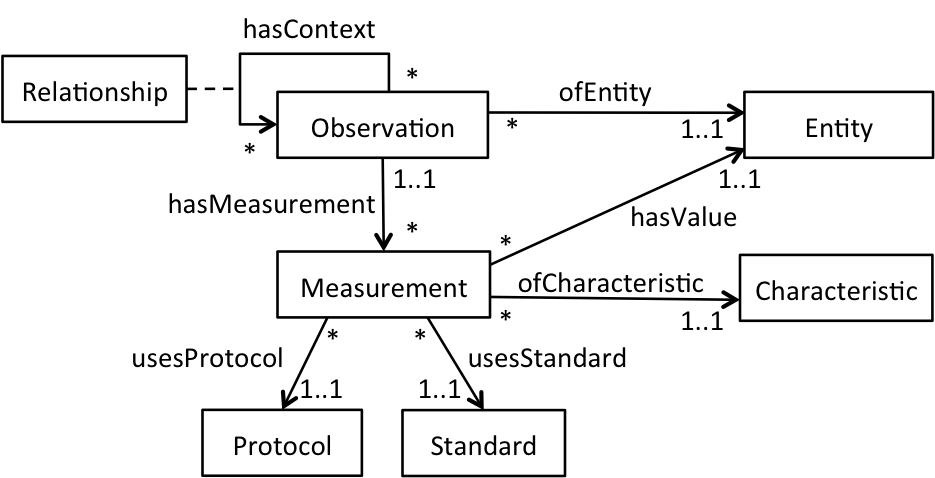
\includegraphics[width=0.5\textwidth]{images/oboe}
  \caption{The main classes and properties of the extensible
    observation ontology (OBOE). While shown here using UML, the model is
    defined using OWL-DL.}
  \label{fig:oboe}
\end{figure}

\begin{figure}
\centering
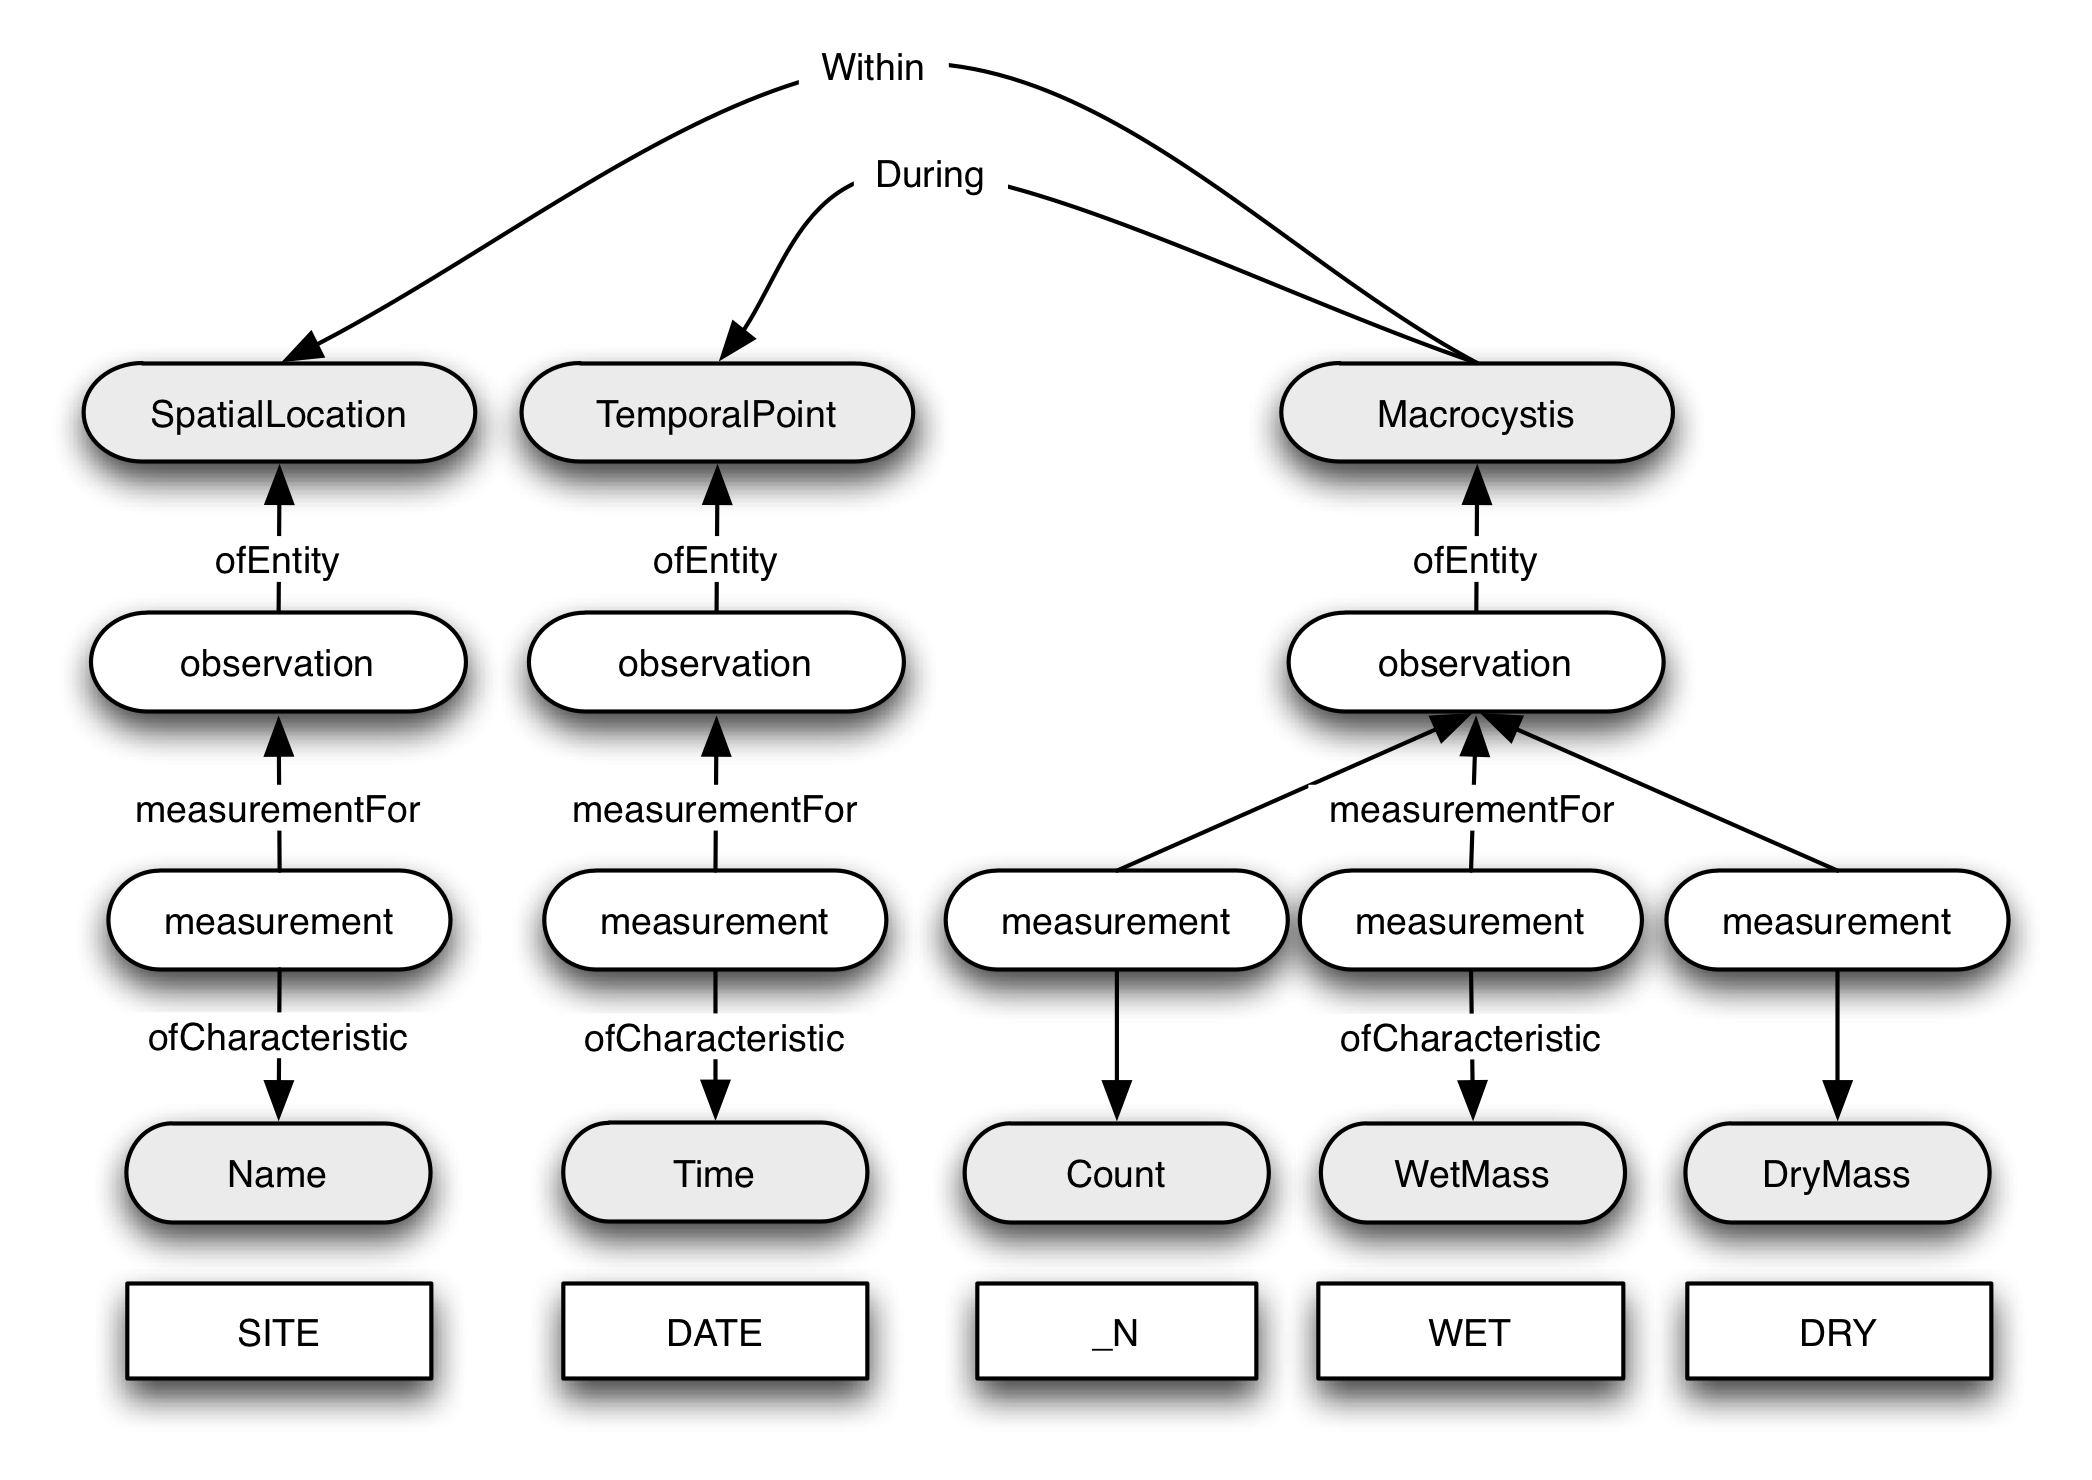
\includegraphics[width=0.5\textwidth]{images/kelp-mass-model.png}
\caption{Partial OBOE annotation for Kelp sampling data. Shaded nodes represent ontological concepts; rectangular nodes are data table attibutes mapped to OBOE characteristics. Measurement standards (e.g., grams) and collection protocols are not illustrated.}
\label{fig:kelp-mass-model}
\end{figure}

%%% Local Variables: 
%%% mode: latex
%%% TeX-master: "main"
%%% End: 

\section{Framework}
\label{sec:framework}

Semtools has focused development effort on three components:
a Java library for accessing and manipulating OBOE ontology extensions and Annotations,
an Annotation plugin for the Morpho metadata editor, and query extensions for the Metacat data catalog.

\subsection{Semantic mediation API}
The SMS API includes ontology management features, annotation manipulation capabilities, and simple concept navigation and visualization widgets. The API is intended to be a centralized toolkit for use in multiple contexts - be they client or server - that abstracts the specifics of any single semantic library. That being said, OWL API primarily underlies the ontology management interface providing RDF/OWL parsing and serialization as well as simple class and property exploration. A Pellet reasoner exposes inferred axioms and relationships that are not explicitly defined in the source ontologies. Inference is particularly powerful when utilizing OBOE Measurement 'templates' that express exactly what (Entity and Characteristic) can be observed and how (Standard and Protocol). 

Annotations are ultimately managed and stored in an opaque local relational database chosen for scalible persistence and query performance; the overhead of in-memory Annotation queries having proven to be prohibitively limiting for large sets of data.

\subsection{Morpho editor plugin}
The semantic editor plugin for Morpho provides a front-end to the SMS API and allows metadata editors to build up semantic Annotations for existing data package descriptions. The editor focuses on a simplictic fill-in-the-blank style interface with reusable, searchable, hierachical concept selection widgets (\figref{fig:morpho-annotation}). The optional plugin seamlessly integrates with a standard Morpho installation augmenting the existing features to provide semantic query capabilities for locating data packages, marking up data packages with semantic Annotations, and saving Annotations locally or to a shared repository where they can be discovered and explored by a broader audience.

\begin{figure}
\centering
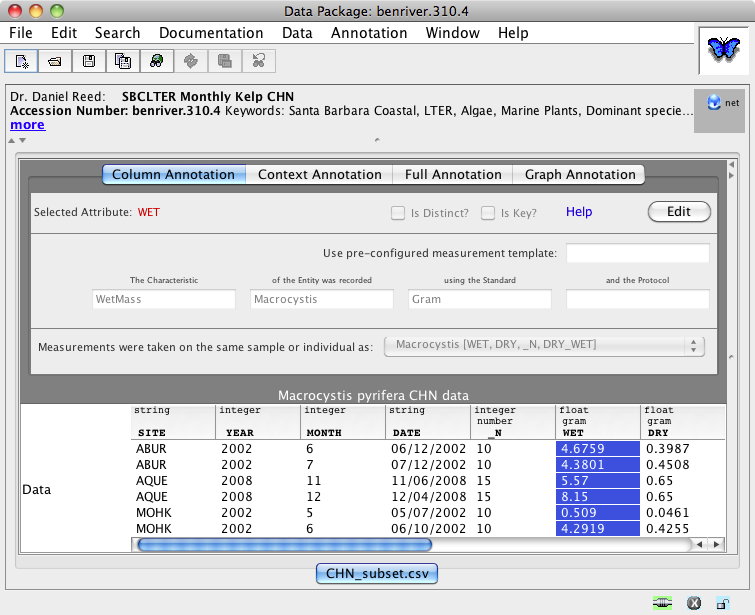
\includegraphics[width=0.5\textwidth]{images/morpho-annotation.png}
\caption{Morpho metadata editor with Semantic plugin. Fill-in-the-blank style editing interface to encourage natural language descriptions. A searchable hierarchical browser is used to select concepts from an ontology.}
\label{fig:morpho-annotation}
\end{figure}

\subsection{Metacat query extensions}
The semantic plugin for Metacat augements existing metadata storage and search by allowing Annotations to be saved and queried alongside the metadata and data that they annotate. In addition to traditional keyword and spatial search criteria, the Metacat plugin allows semantic criteria to be included where they may either increase query recall using term-expansion (i.e. traversing the class subsumption hierarchy) or refine the resultset by limiting matches to datasets that contain the specified observational model (e.g. combinations of OBOE-compatible Entity, Characteristic, or Protocol concepts). The observational model can be leveraged further by materializing the Annotation and data artifact (via the Data Manager Library) into a full OBOE model and inspecting the observational values themselves. 

%%% Local Variables: 
%%% mode: latex
%%% TeX-master: "main"
%%% End: 


\section{Discovery and Integration}
\label{sec:application}

\subsection{Concept query}
The semantic query interface primarily supports locating datasets by how well their observational models match the given criteria. Query criteria largely mirror the structure of an Annotation in that combinations of Entity, Characteristic and Protocol are specified and optionally compounded when increased precision is sought. 
By leveraging the relationships defined and/or inferred from the ontology we are able to increase recall beyond what is possible for simple keyword-based searches (Berkely et al, 20??). Broad queries return direct matches and also n-depth subclass matches. The queries can be quickly honed when using this browsing paradigm which allows rapid exploration of the data repository without the oneous of defining complete observational queries \emph{de novo}. Measurement templates as defined in OBOE compatible ontologies enable a single concept to proxy its constituent parts, namely the valid Characteristics of certain Entities that can be measured with certain Protocols and Standards. This short-hand query generation highlights one of the compelling applications of using OBOE compatible ontologies and can also be leveraged when authoring Annotations.
Using compound semantic query criteria applies a fine-grained filter on the datasets that are returned. Results may include only those datasets that include measurements for a set of specific Characteristics of a particular Entity. Furthermore, a query can specify that those measurements come from precisely the \emph{same instance of that Entity} as belaboured by the authors of the OBOE specification (Schildhauer here somewhere??).

\subsection{Data query}
For even more precise recall, the OBOE model can be partially \emph{materialized} during the query stage after which a data range filter can be applied. Different techniques are available for merging the Annotation with the data that it describes, but for performance reasons a hybrid approach has been adopted in which premliminary search results from a concept-based query are collated and only that subset is materialized. The Data Manager Library is conveniently used to load raw data objects because our corpus is described using EML and the Annotation syntax - both of which inform the correct use of the Data Manager query features. For any data attributes that match the concept query criteria, we then verify that those attributes contain data values within the range specifed by the initial semantic data query (\figref{fig:metacat-query}).

\begin{figure*}
\centering
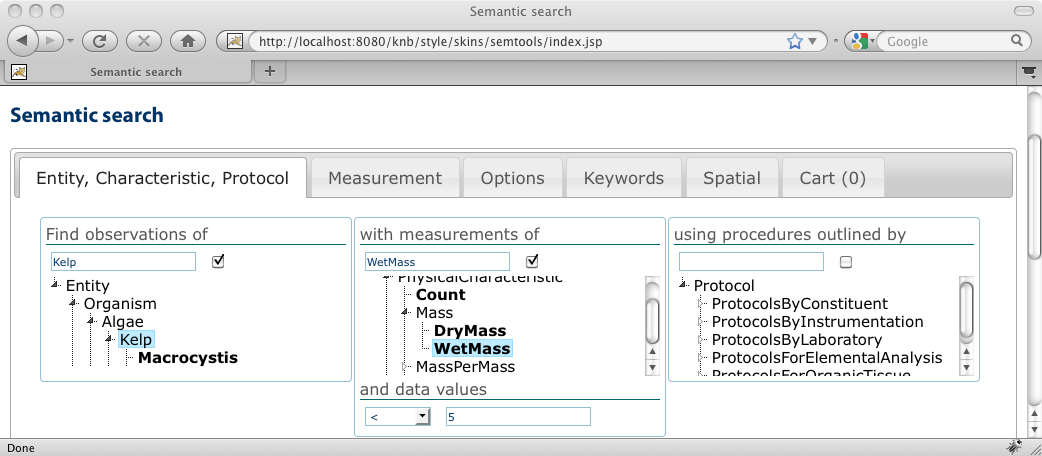
\includegraphics[width=1.0\textwidth]{images/metacat-query.png}
\caption{Semantic data query web interface. Data packages containing observations of Kelp Wet Mass less than or equal to 5 [grams] are returned. Additional search options and compund query criteria can be specified within the other tabs. Matches can be saved in the data cart for later exploration.}
\label{fig:metacat-query}
\end{figure*}

\subsection{Data integration}
The materialization routine used for semantic data queries laid the groundwork for our ongoing data integration pursuits.
In addition to inspecting the data for values within a range and returning the packages that contain a match, the "smart" data integration feature goes further by constructing a synthetic data product that represents the complete results of the query both in terms of the attributes and the values that are returned. Each original data package match may have wildly different syntactic structures (e.g. column number, naming, order) but could share a subset of attributes that are asserted as semantically compatible. These compatible, in-common attributes then become the facets and metrics in the synthetic dataset with their values filtered accordingly (\figref{fig:integration}). While preliminary results have been quite promising - albeit academic - continued development of algorithms for determining compatibility of annotated measurements (e.g. gram and ounce are both mass units) and for mutating measurement values using ontologically-defined conversions (e.g. 1000 milligrams in a gram) will enable more thorough data integration.


\begin{figure}
\centering
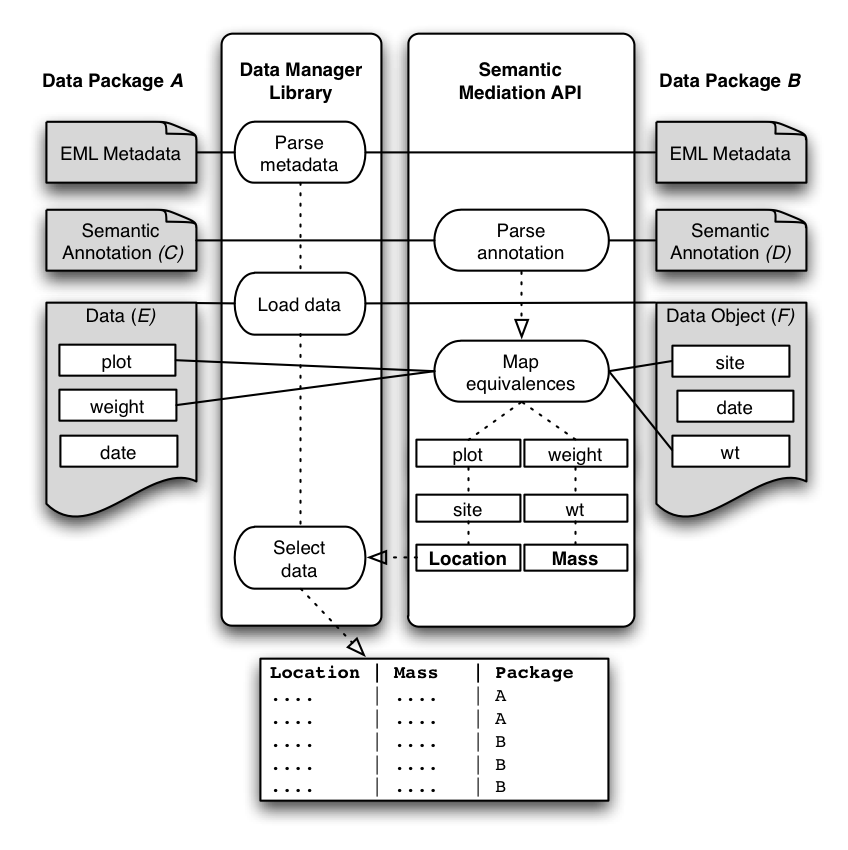
\includegraphics[width=0.5\textwidth]{images/integration.png}
\caption{Data integration query across multiple data packages (A, B).  Annotations (C, D) are used to determine semantically equivalent data attributes contained in the data objects (E, F). Attributes 'plot' and 'site' are considered equivalent measurements of the characteristic 'Location'; attributes 'weight' and 'wt' both map to the same characteristic 'Mass'. The Semantic Mediation API utilizes the Data Manager Library to load and query the source data informed by semantic similarities between the structurally disparate data attributes.}
\label{fig:integration}
\end{figure}

%%% Local Variables: 
%%% mode: latex
%%% TeX-master: "main"
%%% End: 


\section{Related Work}
\label{sec:related}

The need for more semantic mechanisms to describe observational data
has led to many proposals for observational data models (e.g.,
\cite{om, tarboton07:_cuahs_commun_obser_data_model,netcdf}) and
ontologies (e.g.,
\cite{fox09:_ontol,sweet,mungall07:_repres_phenot_in_owl}).  The work
presented here is complementary to these efforts by providing a
concrete set of software components that have been integrated with
popular metadata tools (namely, Metacat
\cite{metacat02:_manag_heter_ecolog_data_using_morph} and Morpho
\cite{berkley01:_metac}) to provide a more uniform, semantic view of
heterogeneous observational data. By extending Morpho and Metacat to
support semantic annotations, these tools can provide additional help
to researchers interested in performing synthetic studies by providing
semantically-enhanced discovery and integration services, which are
largely lacking in many existing environmental information management
frameworks \cite{jones_new_2006}.

Our work on using semantic annotations for data integration is closely
aligned to traditional information integration approaches (e.g.,
\cite{kolaitis05}), where a global mediated
schema is used to (physically or logically) merge the structures of
heterogeneous data sources using mapping constraints among the source
and target schemas. As such, the observational model we employ in our
framework can be viewed as a (general-purpose) mediation schema for
observational data sets.  This schema can be augmented with logic
rules (as target constraints) where semantic annotations are used as
mapping constraints. However, instead of users specifying logic
constraints directly, we provide a high-level annotation language and
user-interface components (through Morpho) that can simplify the
specification of mappings and more naturally aligns with the
observation model.

Annotations are playing a more prominent role in database systems,
e.g., the MONDRIAN system \cite{GeertsKM06} employs an annotation
model and a set of query operators to manipulate both data and
annotations.  However, users must be familiar with the underlying data
structures (schemas) to take advantage of these operators, which is
generally not feasible for observational data in which data sets
exhibit a high degree of structural and semantic heterogeneity. Our
annotation approach used to extend EML is also similar in spirit to a
number of other high-level mapping languages used for data exchange
(e.g., \cite{fagin09:_clio,an06:_build_seman_mappin_datab_ontol}). Our
approach differs by being specifically tailored to the OBOE
observational model, which in turn simplifies the annotation language,
making it in general easier for users to specify annotations for
observational data. Our approach also provides well-defined and
unambiguous mappings from data sets to the observation and measurement
model, which is critical for providing automated, high-quality data
integration services over heterogeneous observational data.

% Some efforts have also been carried out for leveraging annotations,
% e.g., for the discovery of domain-specific data
% \cite{obsdatasearch09,StoyanovichMR10}, however, these approaches are
% largely based on keyword queries, and do not consider structured
% searches. Our work differs in that we consider a highly structured and
% generic model for annotations with the aim of providing a uniform
% approach for issuing structured data-discovery searches.



%%% Local Variables: 
%%% mode: latex
%%% TeX-master: "main"
%%% End: 

\section{Summary}
\label{sec:summary}

The Semtools project has been successful in exploring and codifying
technologies and techniques for applying semantic concepts to
observational data. By providing mechanisms for linking data sets to
ontological terms organized in a high-level observational model (e.g.,
OBOE), these new extensions to Metacat and Morpho help to overcome a
number of limitations in existing metadata management systems that
strive to provide effective data discovery and integration
features. Our close involvement with the SONet Project (Scientific
Observations Network) \cite{sonet} encourages continued use-case
refinement that will inform future semantic tool development and place
an emphasis on intuitive interfaces and incremental adoption. This
varied community of stakeholders is firmly invested in the use of
cutting edge semantic solutions that will ultimately benefit multiple
science disciplines by reducing obstacles to broad data sharing and
innovative reuse.


%%% Local Variables: 
%%% mode: latex
%%% TeX-master: "main"
%%% End: 


% \mypara{Acknowledgements.} ... 

% This work was funded in part through NSF grants \#0743429 and
% \#0753144. We would like to thank Matthew Jones, Benjamin Leinfelder,
% and Margaret O'Brien for their discussions on annotation and
% observational modeling.

\bibliographystyle{IEEEtran}
%\bibliographystyle{alpha}
\bibliography{main}



\end{document}


